% !TEX root = ../ac_paper.tex

\section{Embeddings}

\subsection{Transformers: a review}

Previously an encoder-only transformer was used in

\subsection{Dataset for the GPT model}

We apply sequences of AC moves to the Miller-Schupp series presentations studied in the previous subsection to generate a dataset.
We use Algorithm \autoref{alg:apply_ac_moves} to ensure that the total length of the generated presentations follows roughly a uniform distribution.
(See \autoref{fig:gpt_data}; there, the distribution is roughly uniform with short tails on either side.)
\footnote{Maybe there should be only one histogram in the figure showing combined solved+unsolved statistics.
As it is, I computed separate percentages for each solved/unsolved case.
I should clarify that if I leave the figure as it is.
It is also good to change the total length.
Also change the label of x-axis to something better.}

Algorithm \autoref{alg:apply_ac_moves} generates presentations of increasing lengths in $n$ phases.
In the $i$-th phase, presentations with maximum relator length $l_i$ are generated, where $l_i$ is sampled from a discrete uniform distribution with bounds $l + i l_{\text{inc}} $ and $l + (i+1) l_{\text{inc}}$.
Here, $l$ is the maximum of the lengths of the two relators in the initial Miller-Schupp presentation $R_0$ (and thus the minimum value of maximum relator length in the algorithm), and $l_{\text{inc}}$ is defined in terms of the maximum possible relator length $l_{\text{max}}$ we wish to obtain in the last phase as $l_{\text{inc}} = (l_{\text{max}}-l)/n$.
In the $i$-the phase, $T$ AC moves are applied to a presentation generated in the $(i-1)$-th phase.
In our work, we chose $l_{\text{max}}=128$, $n=128$, $m=12$, and $T=1000$.
\footnote{Specify much earlier in the paper, and here as well, that whenever we apply AC moves, we set a maximum length up to which each relator is allowed to grow.
Any AC move that would result in a presentation of longer relator length acts trivially.
Maybe instead of writing $A \sim \text{AC Moves}$, there should be a notation like $(AC)_l$ when $l$ is specified to be the maximum relator length.}

\begin{algorithm}
	\caption{Generate AC Cousins}\label{alg:apply_ac_moves}
	\begin{algorithmic}
		\Require $R_0$, $l_{\text{max}}$, $n$, $m$, $T$
		\State $L \gets \{ \}$ \Comment{Initiate the list $L$ of all presentations}

		\State $l \gets \max(l_1, l_2)$

		\Comment{Set $l_1$, $l_2$ are the lengths of relators of $R_0$}

		\State $l_{\text{inc}} \gets (l_{\text{max}}-l)/n$

		\Comment{The increment by which the maximum relator length increases in each phase}

		\For {$i = 1, 2, \dots, n$}

		\Comment{Loop over $n$ phases}
		\For {$j = 1, 2, \dots, m$}

		\Comment{Generate $m$ presentations in each phase}
		\State $l_i \sim \mathcal{U}(l + i l_{\text{inc}} , l + (i+1) l_{\text{inc}})$

		\Comment{Set the maximum relator length for $i$-th phase}
		\If{i is 0}
		\State $R \gets R_0$
		\Else
		\State $R \gets L[(i-1) \times m+j]$
		\EndIf

		\Comment{Set $R$ to a presentation of the previous phase if $i > 0$, else set it to the initial presentation $R_0$}


		\For{$k = 1, 2, \dots, T$}

		\Comment{Apply $T$ randomly selected AC-moves}
		\State A $\sim$ AC Moves
		\State $R \gets A \cdot R$

		\EndFor

		\State $L \gets R$

		\Comment{Add the resultant presentation $R$ to $L$}

		\EndFor
		\EndFor
	\end{algorithmic}
\end{algorithm}

The main reason for choosing this algorithm is so that our GPT model sees roughly the same amount of presentations of each length and is, hence, not biased towards shorter or longer presentations.
The final dataset contained 0.8 million (1 million) presentations generated from applying Algorithm \autoref{alg:apply_ac_moves} to BFS-easy (BFS-hard) examples.
Only a small amount (roughly 15 percent) of the original Miller-Schupp presentations remained to be part of this dataset.

\begin{figure}
	\centering
	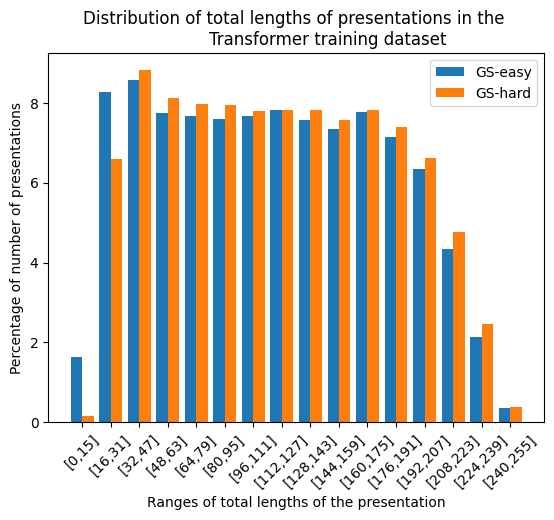
\includegraphics[scale=0.6]{fig/gpt_data_length_distribution.png}
	\caption{Percentage of presentations in various ranges of total lengths.}
	\label{fig:gpt_data}
\end{figure}

The dataset is tokenized by adding two stop tokens that represent the end of two relators of a presentation.
Thus there are six tokens in total: one each for $x$, $y$, $x^{-1}$, and $y^{-1}$ and the two stop tokens.
The tokenized dataset has about 217M tokens, and the distribution of tokens is shown in \autoref{fig:tokens_hist}.
We note that $y$ and $y^{-1}$ appear significantly more often than $x$ and $x^{-1}$ in the unsolved dataset.
This is likely because the BFS-hard examples have higher $n$, and higher $n$ corresponds to more of a presence of $y$ and $y^{-1}$.
Interestingly, this effect remains in the dataset even when we apply thousands of AC moves.
I should investigate this further.

We set aside 10 percent of the data as a validation dataset.

\begin{figure}
	\centering
	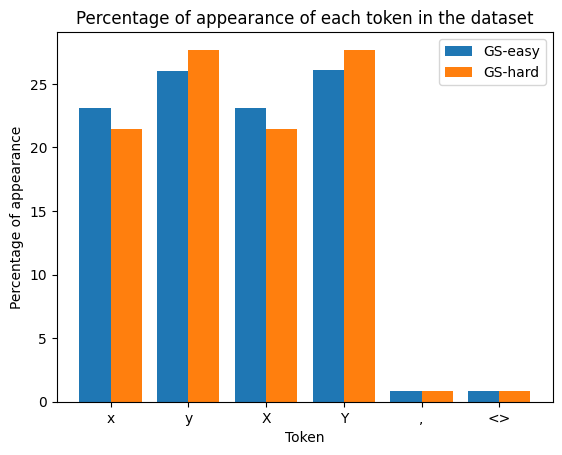
\includegraphics[scale=0.6]{fig/tokens_hist.png}
	\caption{Percentage of appearance of each token in the solved/unsolved datasets.}
	\label{fig:tokens_hist}
\end{figure}

\subsection{Results}
We train a GPT model on the dataset described in the previous subsection.
Given a context of $n$ tokens, a GPT model learns the probability distribution for $(n+1)$-st token.
The extent to which it can make good predictions is measured by a cross-entropy loss defined above.
We trained a model with embedding dimension 512 and 8 layers.
The model is initialized with random weights that assigns an equal probability to each token, thus the initial value of the cross-entropy loss is $-\ln(1/6) \sim 1.7917$.
As the model was trained, we were able to achieve the minimum validation loss of 0.5685.
\footnote{insert a validation loss curve.}

We use the trained model to obtain embeddings of the 1190 Miller Schupp presentations studied above.
To visualize these embeddings, we use t-SNE with distance measured by the cosine of the angle between two embedding vectors and project the embedding space down to two dimensions.
The final result is shown in \autoref{fig:embeddings_tsne}.
We see that the model has clustered together examples with the same $n$.

\footnote{Maybe I should replace 'Solved' and 'Unsolved' with 'BFS-easy' and 'BFS-hard' in all the images.}

\begin{figure}
	\centering
	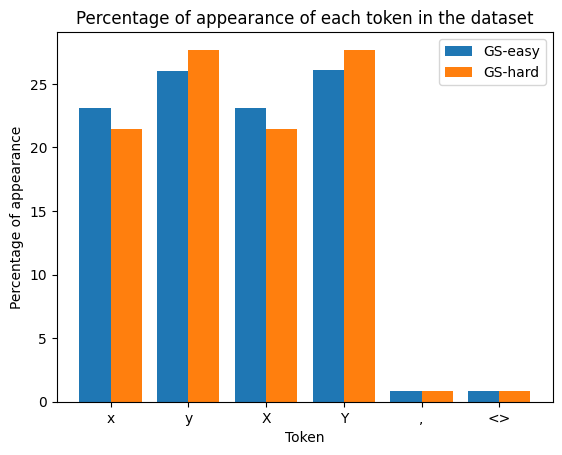
\includegraphics[scale=0.6]{fig/tokens_hist.png}
	\caption{Percentage of appearance of each token in the solved/unsolved datasets.}
	\label{fig:tokens_hist}
\end{figure}

\begin{figure}
	\centering
	\begin{subfigure}[b]{\textwidth}
		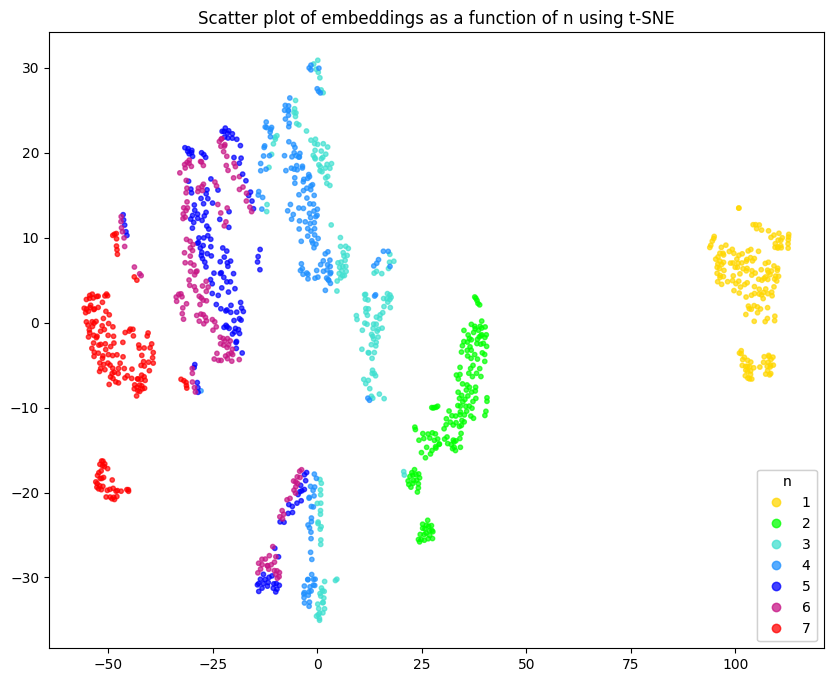
\includegraphics[width=1\linewidth]{fig/embeddings_n.png}
		\caption{Scatter plot of embeddings as a function of $n$ using t-SNE}
		\label{fig:hist_vs_n}
	\end{subfigure}%
	%add desired spacing between images, e. g. ~, \quad, \qquad etc.
	%(or a blank line to force the subfigure onto a new line)

	\begin{subfigure}[b]{\textwidth}
		\centering
		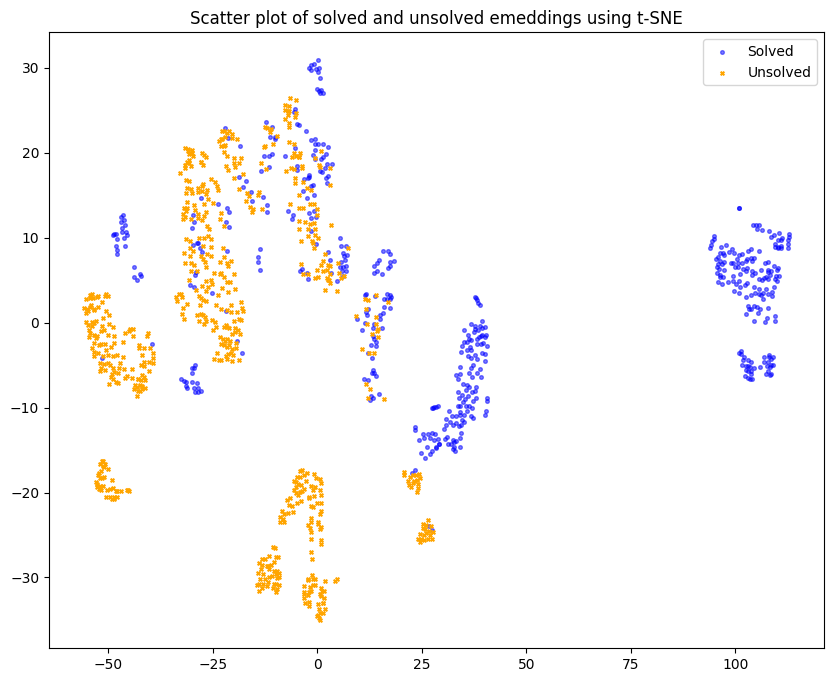
\includegraphics[width=1\linewidth]{fig/embeddings_easy_vs_hard.png}
		\caption{Scatter plot of BFS-easy and BFS-hard examples using t-SNE}
		\label{fig:hist_vs_length}
	\end{subfigure}
	\caption{Projection of embeddings to a plane using t-SNE with cosine similarities}\label{fig:embeddings_tsne}
\end{figure}


\fixme{Is one way to interpret this result that the application of  BFS moves takes us far away from the initial presentation, but it still remembers which presentations should be hard vs easy?}